\chapter{Science Is Elementary - Overview}

Science Is Elementary is a series of educational video games developed by The Lightspan Partnership. There are ten videos in total contained over the entirety of the three CD's: four for the Science Is Elementary 1, and then three each for Science Is Elementary 2 and 3. Each of the videos in the series is designed to give a brief overview of an area of science, with titles such as "Let's Explore Plants" and "Let's Explore Weather and the Seasons".

Similar to some of the other titles from Lightspan, there is no additional content to these titles, and they are purely educational videos. The videos are designed to be used in a classroom setting, with the teacher able to pause the video at any time to discuss the content with the students.

Each series of videos follows a similar format: an introduction to the topic by a young girl, who provides a brief overview of the topic in front of the camera (who appears in all of the videos), followed by a series of clips showing the topic in action, usually with additional narration by the young girl, and occassionally featuring other children as well. This is then followed by a classroom section, in which a teacher provides a more in-depth look at the topic, discussing the subject in more detail with his or her students. Afterwards, another video clip is shown, with the same young girl at the beginning highlighting the key points of the topic, before finally another shot of the young girl is shown, who provides a brief conclusion to the topic. In most of these videos she ends with the phrase "You try it!" - all except for "Let's Explore Light and Shadows", which is the final video for Science Is Elementary 1. Although a text box appears on the screen at the end of the video that says "You try it", the young girl doesn't speak this.

\begin{figure}[H]
    \centering
    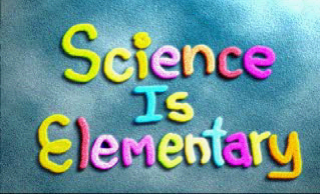
\includegraphics[width=0.5\textwidth]{./Games/ScienceIsElementary/Images/ScienceIsElementaryLogo.png}
    \caption{Science is Elementary Logo}
\end{figure}

Based off the credits revealed at the end of each of the videos, it appears that the vast majority of the schools that were involved in the creation of these videos were based in and around Chicago, Illinois, including Park View School in Morton Groves (just outside of Chicago), and Sacred Heart Schools, a private school in Chicago. In addition, each of the videos were produced with the assistance of a number of science consultants: Denise E. Lessow, Ed.D., and Eric Worch, both from the Indiana University School of Education.

At the end of each video, after the credits have rolled, a short advertisement from the AIT (the Agency for Instructional Technology) was show, advertising corresponding Teacher Guides to go along with the videos. As well, the videos were overall produced by a company called General Learning Video, who themselves worked with a number of companies in the United States in order to create educational videos.

In addition to Vimm's Lair, the only way that I was able to obtain information regarding this series was from the YouTube Channel [Game Cart Classics](https://www.youtube.com/@gamecartclassics), who had managed to upload all three of the CD's to their channel in full. Apart from these sources, and the physical disks there are no other references to go by.

Unfortunately there isn't much information available about the Science Is Elementary series, and it is unknown how well the series was received by schools and teachers. In addition to this, given the limited content for this, there is very little information that can in fact be provided about the series.